
\documentclass[titlepage]{article}
 \usepackage[utf8]{inputenc}
\usepackage{listings}
\usepackage{verbatim}
\usepackage{float}
\usepackage{graphicx}
\graphicspath{ {imagenes/} }
 \usepackage{xcolor}
 \definecolor{RoyalBlue}{cmyk}{1, 0.50, 0, 0}
\usepackage{amsmath}
\lstset{language=Java,
	keywordstyle=\color{RoyalBlue},
	basicstyle=\scriptsize\ttfamily,
	commentstyle=\ttfamily\itshape\color{gray},
	stringstyle=\ttfamily,
	showstringspaces=false,
	breaklines=true,
	frameround=ffff,
	frame=single,
	rulecolor=\color{black}}


 

% Datos de la portada
\begin{document}
	\begin{titlepage}
		\begin{center}
			\vspace*{1cm}
			\date{} % para que no aparezca la fecha la dejo en blanco
			\Huge
			\textbf{Practica 2: Algoritmos Genéticos y Meméticos}
			
			\vspace{0.5cm}
			\LARGE
			Metahurística
			
			\vspace{1.5cm}
			
			\textbf{José Manuel Pérez Lendínez}
			\textbf{26051613-L}\newline
			
			\textbf{jmplz14@correo.ugr.es}		

					
			\textbf{Grupo 1 curso 18/19}
			

			
		\end{center}
	\newpage
	\tableofcontents
	\newpage
	\end{titlepage}
	\section{Descripción del problema}
	 El problema se basa en optimizar la clasificación de nuevos elementos a partir de dos particiones. La particiones de entrenamiento y la partición de test.
	 
	Tendremos un conjunto de datos que dividiremos en 5 particiones, 4 para entrenamiento y una para test. La partición de test ira rotando hasta que todas pasen por test una vez. 
	
	Los conjuntos de datos vendrán dados por una clase y un conjunto de características. Se representarán como un vector con la siguiente estructura.
	\begin{center}
		$(x_1, x_2, ... , x_n, y)$
	\end{center}

	Donde las x corresponde a las características y la y a la clase que pertenece ese elemento.
	
	El objetivo sera ser capaces de acertar con el vector de características a la clase que pertenece. Para ello entrenaremos nuestro modelo con los datos de entrenamiento y usaremos los datos de test para ver si el modelo da resultados mas o menos acertados.
	
	El clasificador tendrá que ser capaz de adivinar la clase utilizando la distancia a los datos de entrenamiento mas cercanos a la muestra elegida de los datos de test. Esta técnica se conoce como k-vecinos mas cercanos y sera la utilizada en todos nuestros algoritmos. Nosotros usaremos una k=1 por lo que solo buscaremos el vecino mas cercano para clasificar sin tener en cuenta a el mismo como vecino.
	
	Al trabajar con datos reales sera muy difícil llegar a la solución exacta por lo que se buscaran aproximaciones.
	
	Para esto utilizaremos tres metahurísticas que explicaremos a continuación y que son:
	\begin{enumerate}
		\item Algoritmo genético generacional
		\item Algoritmo genético estacionario
		\item Algoritmo memético
	\end{enumerate}
	\newpage
	
	\section{Aplicación de los algoritmos }
	 En esta parte se explicaran la representación del problema de una forma mas completa y las características comunes que tienen todos los algoritmos.
	 
	 \subsection{Descripción de la representación y calculo de distancias}
	 
	 Para representar los datos usaremos matrices de numpy para los datos, que tendrán la siguiente estructura después de cargarlos desde los fichero.
	
	\[
	datos =
	\begin{bmatrix}
	x_{1,1} & x_{1,2} & ... & x_{1,j} & y_1 \\
	. & . & . & . & . \\
	. & . & . & . & .\\
	x_{i,1} & x_{i,2} & ... & x_{i,j} & y_i
	\end{bmatrix}
	\]
	Esta matriz tendrá que ser normalizada la parte de los datos (las x) entre [0,1] para realizar con ella los cálculos de distancias para ver cual es el vecino mas cercano.
	
	Para los algoritmos RELIEF y para la búsqueda local necesitaremos un vector de pesos que se representara de la siguiente manera:
	$$
		(w_1, w_2, ..., w_j)
	$$
	Este vector sera utilizado para ponderar la importancia de las distintas características de nuestros problemas. El vector tendrá unos valores acotados entre [0,1] y tendremos en cuenta que los valores menores que 0.2 no se utilizara para calcular las distancias en la clasificación. Esto restara importancia a las variables que tengan una ponderación muy baja y que podrían introducir ruido.
	\newline
	
	En esta practica añadimos también una nueva representación a tener en cuenta para los nuevos algoritmos. Los algoritmos genéticos y meméticos costan de unas poblaciones que tendremos que almacenar para ir trabajando con estas. Cada individuo de la población sera un vector de pesos como los mencionados anteriormente. La representación de la población necesita dos características, los vectores de pesos y el valor de la función objetivo para cada individuo.
	
	Para esto usaremos una matriz para almacenar cada individuo de la población y un vector para el valor de la función objetivo para cada individuo de la población.
	
	\[
	Poblacion =
	\begin{bmatrix}
	w_{1,1} & w_{1,2} & ... & w_{1,j} \\
	. & . & . & . \\
	. & . & . & .\\
	w_{i,1} & w_{i,2} & ... & w_{i,j}
	\end{bmatrix}
	\]
	
	$$
	eval\_poblacion = (valor_1, valo_2, ..., valor_i)
	$$
	\newline
	
	
	

	
	

	
	
	\subsection{Calculo de la tasa de reducción}
	La tasa de reducción vendrá dada por la cantidad de pesos de nuestro vector w que sean inferior a 0.2 de forma que usaremos el siguiente pseudónimo para calcularla.
	La formula de la tasa de reducción es la siguiente:
	$$
		tasa_reduccion = 100 \frac{nº\ de\ w_j < 0.2}{w.size}
	$$
	El pseudocódigo seria el siguiente:
	\begin{lstlisting}
	num_reducciones = 0
	for i in pesos
		if pesos < 0.2
			num_reducciones++
	end
	tasa_reduccion = 100*(num_reducciones / pesos.size)
	
	\end{lstlisting}
	
	La implementación con python es muy sencilla y se relizal en una linea: 
	
	\subsection{Calculo de la tasa de clase}
	La tasa de clase nos dará el porcentaje de acierto a la hora de entrenar nuestro modelo. Para ello utilizamos la siguiente formula:
	$$
	tasa_clase = 100 \frac{nº\ de\ istancias\ bien\ clasificadas}{nº\ instancias\ totales\ en\ test}
	$$
	Para saber si una instancia esta bien clasificada se usara el algoritmos de 1-nn vecino mas cercano que explicaremos mas adelante.
	El pseudocodigo para calcular la tasa de clase seria:
	
	\begin{lstlisting}
	num_aciertos = 0
	for i in test
		clase_clasificado = clasificador_1NN(i,pesos)
		if clase(i) == clase_casificado
			num_aciertos += 0
	end
	tasa_clasificacion = 100*(num_aciertos / Y_test.size)
	\end{lstlisting}
	
	\subsection{Función de evaluación}
	La función de evaluación es la encargada dar un valor numérico que representara lo bueno que es nuestro clasificador. Para ello utiliza tanto la tasa de reducción como la tasa de clase y un valor $\alpha$. 
	
	La formula es la siguiente:
	$$
	F(pesos) = (tasa\_clase(pesos) + tasa\_reduccion(pesos)) / 2
	$$ 
	
	 Esto hará que le demos la misma importancia la tasa de reducción y a la tasa de clase a la hora de ver como ajustan los datos. No voy a poner el pseudocódigo porque simplemente es implementar es función sin ninguna complicación mas.
	

	\subsection{Función evaluación para la búsqueda local}
		La implementación utilizada en es la siguiente:
	
	\begin{lstlisting}
	def evaluate(weights, X, y):
		X_transformed = (X * weights)[:, weights > 0.2]
		kdtree = KDTree(X_transformed)
		neighbours = kdtree.query(X_transformed, k=2)[1][:, 1]
		accuracy = np.mean(y[neighbours] == y)
		reduction = np.mean(weights < 0.2)
		return 100*accuracy,reduction*100,100*(accuracy + reduction) / 2
	\end{lstlisting}
	
	Tengo que darle las gracias a Antonio Molner que compartió esta función para que pudiéramos utilizarla. Gracias a KDTree se puede buscar rápidamente a los vecinos más cercanos de cualquier punto.
	Se consigue el leave-one-out gracias a que en el kdtree utilizamos k=2 para quedarnos con los dos vecinos mas cercanos y a continuación con las funciones para array de python nos quedamos con la ultima columna que sera la que no contenga a si mismo.
	\subsection{Generación de la población inicial}
	
	Para esto se ha usado una distribución aleatoria uniforme con la que  inicializaremos los pesos de cada individuo de la población. 
	Esto lo hacemos con una simple orden en python. 
	$$
		Poblacion = np.random.uniform(0,1,(num\_individuos, num\_genes))
	$$ 
	
	Num\_individuos representa el tamaño de población que tendremos y el num\_genes el número de características que tienen nuestros datos.
	
	Cuando se tiene generada los cromosomas de una poblacion necesitamos evaluarlos para saber su función objetivo. Esto lo hacemos mediante la siguiente función.
	
	\begin{lstlisting}
function evaluarPobalcion(X, y, poblacion[][])
	//array donde almacenaremos los valores de la funcion objetivo.
	valores = [0,0,..,0]
		
	//tamano_poblacion representa el numero de individuos que contiene esta.
	for i in [0,tamano_poblacion]
		valores[i] = evaluate(poblacion[i], X, y)
	end
		
	return valores
			
end
	\end{lstlisting}
	\newpage
	
	\subsection{Torneo binario}
	
	El torneo binario sera el método mediante el que elegiremos dentro de una poblacion los padres que pasaran a la siguiente generación.
	Se basa en enfrentar los individuos de la poblacion actual por parejas y quedarnos con el que mayor función objetivo tenga. 
	
	En nuestro caso pasaremos a la función de torneo binario la poblacion actual, sus valores de función objetivo y el número de enfrentamientos que tendremos. Por cada enfrentamiento que se de saldrá un vencedor que permanecerá en la poblacion durante la siguiente generación y el perdedor sera eliminado. 
	
	La selección de los padres a enfrentar se hará con dos enteros aleatorios que representaran los padres de la poblacion a enfrentar.
	\begin{lstlisting}
function torneoBinario(poblacion,valores,num_torneos)
	nueva_poblacion = matriz[num_torneos][num_genes]
	nuevos_valores = array[num_torneos]
	
	for i in [0,num_torneos]
		padre0 = random_entero(0,numero_cromosomas_poblacion - 1)
		padre1 = random_entero(0,numero_cromosomas_poblacion - 1)
		
		if valores[padre0] > valores[padre0]
			nueva_poblacion[i] = poblacion[padre0]
			nuevos_valores[i] = valores[padre0]
		else
			nueva_poblacion[i] = poblacion[padre1]
			nuevos_valores[i] = valores[padre1]
		end
		
		
	end
	return nueva_poblacion, nuevos_valores
end
	\end{lstlisting}
	
	\subsection{Cruce BLX}
	Se basa en mediante dos cromosomas de la poblacion $\mathrm{C}_{1}=\left(\mathrm{c}_{11}, \ldots, \mathrm{c}_{1 \mathrm{n}}\right)   \mathrm{y}  \mathrm{C}_{2}=\left(\mathrm{c}_{21}, \ldots, \mathrm{c}_{2 \mathrm{n}}\right)$ y se crean dos hijos. Para esto cogemos cada gen de los cromosomas $C_1$ y $C_2$ y se generan dos nuevos que seran introducido en los hijos. Los nuevos genes de hijos se calculan de la siguiente manera.
	
	\begin{enumerate}
		\item Seleccionamos el mayor y el menor de los genes elegidos del $C_1$ y $C_2$.
		 
		$$
		C_{\max }=\max \left\{\mathrm{c}_{11}, \mathrm{c}_{2 \mathrm{l}}\right\}
		$$
		$$
		\mathrm{C}_{\mathrm{min}}=\min \left\{\mathrm{c}_{1 \mathrm{i}}, \mathrm{c}_{2 \mathrm{j}}\right\}
		$$
		\item Nos quedamos con la diferencia entre el mayor y el menor.
		$$
		\mathrm{I}=\mathrm{C}_{\max }-\mathrm{C}_{\min }, \alpha \in[0,1]
		$$
		\item Con esto generamos dos aleatorios en el rango 
		$$
		\left[\mathrm{C}_{\min }-\mathrm{I} \cdot alpha, \mathrm{C}_{\max }+\mathrm{I} \cdot alpha \right]
		$$
		
		Los dos aleatorios generados pasaran a ser los genes de los hijos.
		
	\end{enumerate} 
	Esto se realizara tantas veces como genes tienen los padres.
	
	
	
	\begin{lstlisting}
function cruceBlx(C1, C2, alpha)
	hijo1 = array[numero_genes]
	
	hijo2 = array[numero_genes]
	
	for i in range [0,numero_genes]
		cmin = menor de C1[i] y C2[i]
		cmax = mayor de C1[i] y C2[i]
		I = cmax-cmin
		
		hijo1[i] = random(cmin-I*alpha, cmax+I*alpha)
		hijo2[i] = random(cmin-I*alpha, cmax+I*alpha)
		
		if hijo1[i] > 1: hijo1[i] = 1
		if hijo2[i] > 1: hijo2[i] = 1
		if hijo1[i] < 0: hijo1[i] = 0
		if hijo2[i] < 0: hijo2[i] = 0
		
	end
	
	return hijo1,hijo2
	
	
end

	\end{lstlisting}
	
	\subsection{Cruce aritmético}
	
	En este caso he realizado un cambio respecto al dado en las diapositivas para poder generar dos hijos por cada padre en vez de uno.
	
	En vez de realizar la media aritmética como nos indican las diapositivas de practicas, realizo una media ponderada. De esta forma obtengo dos hijos por cada cruce.
	
	\begin{enumerate}
		\item Genero un vector de números aleatorios del mismo tamaño que los padres. Los valores aleatorios estarán entre $[0,1)$
		
		\item Despues para cada gen de los padres realizo la media ponderada y relleno los hijos con los resultandos de estos.
		
		$$
		hijo1[i] = C1[i] * ponderado[i] + C2[i] * (1-ponderado[i])
		$$
		$$
		hijo2[i] = C1[i] * (1-ponderado[i]) + C2[i] * ponderado[i]
		$$
		
		
	\end{enumerate} 
	Esto se realiza tantas veces como genes tienen los cromosomas.
	\newpage
	
	
	\begin{lstlisting}
function cruceAritmetico(cromosoma1,cromosoma2)
	ponderado = array[num_genes]
	ponderado = Se rellena con aleatorios en el rango [0,1)
	
	hijo1 = array[numero_genes]
	hijo2 = array[numero_genes]	
	
	for i in [0,num_genes]
		hijo1[i] = cromosoma1[i] * ponderado[i] + cromosoma2[i] * (1-ponderado[i])
		hijo2[i] = cromosoma1[i] * (1-ponderado[i]) + cromosoma2[i] * ponderado[i]
	end
	
	return hijo1, hijo2
end
	\end{lstlisting}
	
	\subsection{Cruce Rand}
	En este caso se seleccionan tres padres para realizar la operación de cruce. La operación se realizara sobre un cuarto individuo de la poblacion. Los tres padres no podrán coincidir con el 4 elemento. Se tendrá una probabilidad para que se acepte el gen de la recombinación de los tres padres(En nuestro caso un 0.5), si no se cumple la probabilidad nos quedaremos con el gen del cuarto individuo. Para obtener los genes de los tres padres que se introducirán al cuarto individuos se realizara la siguiente operación. 
	
	$$
	V_{i, G}=X_{r I, G}+0.5 \cdot\left(X_{r 2, G}-X_{r 3, G}\right)
	$$
	
	El pseudocódigo es el siguiente:
\begin{lstlisting}
function cruceRand(padre_1, padre_2, padre_3, cuarto_individuo)
	nuevo_individuo = (0,...,0)
	for j in (0,size(cuarto_individuo)-1)	
		if rand(0,1) < 0.5:
			nuevo_individuo[j] = padre_1[j] + 0.5 * (padre_2[j] - padre_3[j])
			if nuevo_individuo[j] < 0
				nuevo_individuo[j] = 0
			end
			
			if nuevo_individuo[j] > 1
				nuevo_individuo[j] = 1
			end
		else
			nuevo_individuo[j] = cuarto_individuo[j]
		end
		
	end
	
	

end
\end{lstlisting}	
	\subsection{Cruce Current to Best}
	En este caso se seleccionan dos padres para realizar la operación de cruce. La operación se realizara sobre un tercer individuo de la poblacion. Los dos no podrán coincidir con el tercer individuo. Se tendrá una probabilidad de 0.5 de cruce. En este cruce se utilizara también el mejor elemento de la poblacion para el cruce. Se realizara la siguiente operación con los elementos. 
	
	$$
	V_{i, G}=X_{i, G}+0.5 \cdot\left(X_{b e s t, G}-X_{i, G}\right)+0.5 \cdot\left(X_{r l, G}-X_{r 2, G}\right)
	$$
	
	El pseudocódigo es el siguiente:
	\begin{lstlisting}
function cruceCurrentToBest(padre_1, padre_2, mejor_individuo, tercer_individuo)
	nuevo_individuo = (0,...,0)
	for j in (0,size(tercer_individuo)-1)	
		if rand(0,1) < 0.5:
			nuevo_individuo[j] = tercer_individuo[j] + 0.5 * (mejor_individuo[j] - tercer_individuo[j]) + 0.5 * (padre_1[j] - padre_2[j])
			if nuevo_individuo[j] < 0
				nuevo_individuo[j] = 0
			end
	
			if nuevo_individuo[j] > 1
				nuevo_individuo[j] = 1
			end
		else
			nuevo_individuo[j] = tercer_individuo[j]
		end
	
	end
	
	
	
end
	\end{lstlisting}
	
	\subsection{Mutar gen}
	La mutación se realiza en una posición del cromosoma. Ha esta posición se le suma un aleatorio generado con una distribución normal con $\sigma = 0.3$. Se tiene que controlar que la mutación no queda por encima de 1 o por debajo de 0
	
	\begin{lstlisting}
fucntion mutarGen(cromosoma, posicion)
	valor_mutacion = distribucion_normal(0.0, 0.3)
	cromosoma[posicion] += valor_mutacion
	
	if cromosoma[posicion] > 1; cromosoma[posicion] = 1	
	if cromosoma[posicion] < 0; cromosoma[posicion] = 0
	
	return cromosoma

end
	\end{lstlisting}	
	\newpage
	
	\section{Explicación de los algoritmos}
	En esta sección explicaremos los tres algoritmos que hemos utilizado para obtener los datos de clasificación.
	
	\subsection{Algoritmo del vecino mas cercanos 1-NN}
	El algoritmos 1-NN o vecino mas cercano se entrena con las particiones de entrenamiento para poder clasificar las entradas de la partición de test. Se basa en el buscar el vecino mas cercano de las muestras de entrenamiento para una muestra de test. De este modo calcula la distancia euclidea de cada elemento de entrenamiento con respecto a un elemento de test. Selecciona el que mas se acerca y mira la clase de este. Si la clase coincide con la clase del elemento de entrenamiento se da como acertado.
	
	En mi caso he implementado dos uno para obtener los datos del 1-NN en el que no necesitamos pasarle vector de pesos y que utilizo KNeighborsClassifier de la librería de python sklearn como clasificador.
	
	El pseudocódigo es el siguiente:
	\begin{lstlisting}
	def K-NN(datos_train,datos_test){
	
		X_train = datos(datos_train)
		X_test = datos(datos_test)
		Y_train = datos(datos_train)
		Y_test = clase(datos_test)
		
		num_aciertos = 0
		#esto indica al clasificador que buscara uun unico vecion cercano
		clasificador = crearClasificador(n=1)
		clasificador = clasificador.entreno(X_train,Y_train)
		
		num_elementos = getNumeroElementos(X_test)
		
		for i in [0,num_elementos]
			clase = clasificador.predice_clase(Y_test[i])
			if clase == Y_test[i]
				num_aciertos += 1
			end
		end
		tasa_acierto = 100 * (num_aciertos / Y_test.size)
		
		#como no trabaja con pesos el valor de tasa_reduccion sera 0
		return tasa_acierto,funcionObjetivo(tasa_acierto,0)
	}
	\end{lstlisting}
	\newpage
	
	\subsection{Algoritmo RELIEF}
	El algoritmo RELIEF es una solución greedy que se basa en buscar el enemigo y vecino mas cercano para para mejorar el vector de pesos. El vector de pesos se inicia a 0.
	
	La formula utilizada para calcular el nuevo vector de pesos es la siguiente:
	$$
		pesos = pesos + | e_i-e_e | - |e_i - e_a|
	$$
	Esto se realiza para cada elemento del conjunto de entrenamiento. 
	
	Una vez terminado se calcula la función objetivo clasificando mediante uno-NN pero antes hay que normalizar el vector de pesos por si alguno ha sobrepasado el uno o es menor que 0. De esta manera se coloca a 0 los menos que este y nos quedamos con el valor mayor del vector para normalizar respecto a este todos los valores. 
	\newpage
	\begin{lstlisting}
	def RELIEF(X_train,Y_train,X_test, Y_test)
		num_elementos = getNumeroElementos(X_test)
		pesos = zeros(num_elementos)
		
		#creo una matriz de distancia para no tener que 
		#estar calculando consantemente distancias para calcular 
		#y repetir calculos
		distancias = disntacia_euclidea(X_train)
		
		#Recorremos la matriz de distancia comparando
		for i in [0,num_elementos]
			mejor_enemigo = int()
			valor_enemigo = max_float
			mejor_amigo = int()
			valor_amigo = max_float
			
			for j in [0,num_elementos]
			
				if Y_train[i] == Y_train[j]
					
					if valor_amigo < distancias[i][j]
						#Se evita que se el mimso el mejor amigo
						if i != j
							mejor_amigo = j
							valor_amigo = distancias[i][j]
						end
						
					end
					
				else
				
					if valor_enemigo < distancias[i][j]
						mejor_enemigo = j
						valor_amigo = distancias[i][j]
					end
					
				end	
				
			end
			
			pesos = pesos + |X_train[i]-X_train[mejor_enemigo]| -
			|X_train[i]-X_train[mejor_amigo]|
		end
		
		#normalizamos el vector de pesos si es menor 
		
		max = obtenerMayor(pesos)
		
		for i in peso
			if i < 0
				i = 0
			else
				i = i / max
		end
		
		return uno-nn(X_train,Y_train,X_test,Y_test,pesos)
		
	end	
	\end{lstlisting}
	\newpage
	\subsection{Algoritmo de Búsqueda Local}
	En la búsqueda local iremos generando vecinos por mutación hasta un máximo de 15000.
	El pseudocódigo para la mutación es el siguiente. En mi caso he usado la librería randon de numpy. Si el peso supera 0 o 1 se trunca el peso.
	
	\begin{lstlisting}
	def mutacion(posicion,pesos)
		Z = np.random.normal(0.0, 0.3, None)
		pesos[posicion] += z
		if pesos[posicion] > 1 
			peso[posicion] = 1
		end 
		if pesos[posicion] < 0
			peso[posicion] = 0
		end 
			
		return pesos
	end
	\end{lstlisting}
	
	El valor 0.3 es la varianza que utilizaremos para la mutación.
	Para generar el primer vector de pesos se tiene que realizar de forma aleatoria con valores entre [0,1]. Para eso utilizo también la librería numpy.random de python con la opción rand que genera valores entre 0 y 1
	
	\begin{lstlisting}
	def generar_vector(num_valores)
		pesos = np.random.rand(num_valores)
		return pesos
	end
	\end{lstlisting}
	
	La búsqueda local ira mutando un componente del vector y quedara este si mejora los valores que el anterior. Si no se da la mejora volverá al anterior y mutara el siguiente valor. Por cada fallo en la mutación se contara un erro de mejora. Si se obtiene 20*n errores en la mejora de forma consecutiva se para la búsqueda. El valor n corresponde al número de características que tienen un elemento de nuestro dataset.
	
	De esta forma ya tenemos dos criterios de parada, el generar 15000 vecionos o no mejorar en 20*n mutaciones de forma consecutiva.
	
	Para mejorar un poco los tiempos antes de realizar una comprobación de si los pesos son mejores que los anteriores miro dos cosas.
	
	La primera es que si antes de mutar una posición del vector de pesos esa posición era menor que 0.2 y al mutar sigue siendo menor que 0.2, sabemos que no tendrá mejora, por lo que no realizamos la comprobación.
	
	La segunda opción que nos asegura que no se da mejora es cuando al mutar un gen el valor anterior era igual que el valor mutado. Esto parece poco probable pero cuando el valor de ese peso antes de la mutación ya era 1 si nos sale en la mutación un valor positivo no mejorara ese 1 puesto que es el valor máximo. En ese caso tampoco hago la comprobación de mejora.
	
	El pseudocódigo es el siguiente;
	\newpage
	\begin{lstlisting}
	def BL(X_train,Y_train,X_test, Y_test)
		w = generar_vector(getNumeroCaracteristicas(X_train))
		pos_w = 0
		num_veciones = 0
		sin_mejora = 0
		
		#Se comprueba el valor de la solucion
		tasa_clase, tasa_reduccion = evaluate(train_datos, train_clases, w)
		
		funcion_mejora = funcionObjetivo(tasa_clase,tasa_reducion)
		
		mejor_valor_w = funcion_mejora
		mejor_w = w
		mejor_tasa_clase = tasa_clase
		mejor_tasa_reduccion = tasa_reduccion
		
		while num_vecions < 15000 y sin_mejora < 20 * num_pesos
			num_veciones += 1
			anterior_peso = w[pos_w]
			pesos = mutacion(pos_w,pesos)
			
			#comprobamos si hay que calcular la mejora
			if comprobarSiCalculamosMejora(anterior_peso,w[pos_w]):
				w[pos_w] = anterior_peso
				sin_mejora += 1	
				
			else
				tasa_clase, tasa_reduccion = evaluate(train_datos, train_clases, w)            
				funcion_mejora = funcionObjetivo(tasa_clase,tasa_reducion)
				
				
				if mejor_valor_w < funcion_mejora:
					
					#Si mejora actualizamos los mejores valores
					mejor_w = w
					mejor_valor_w = funcion_mejora
					mejor_tasa_clase = tasa_clase
					mejor_tasa_reduccion = tasa_reduccion
					sin_mejora = 0
				
				
				else:
					#volvemos al valor anterior y contamos una pasada sin mejora
					w[pos_w] = anterior_peso
					sin_mejora += 1
				end
			
			end
			
			
			pos_w = (pos_w+1) % size(w)
		
		end
		
		return uno-nn(X_train,Y_train,X_test,Y_test,pesos)
	end
	\end{lstlisting}
	\subsection{Algoritmo genético generacional}
	El AGG (algoritmo genético generacional) parte de una poblacion inicial y en cada época cambia completamente la población actual por una población nueva. Esto se realiza mediante el proceso de selección en el que compiten los padres por continuar en la poblacion. En este caso usamos el torneo binario para realizar esta selección. Los individuos con mejor función objetivo tendrán mas opciones de ganar un combate y quedar en la nueva poblacion. Los individuos que competirán se eligen aleatoriamente. Si se tienen N individuos en la poblacion se realizaran N*2 torneos. 
	
	Después realizamos los cruces entre padres para generar nuevos hijos. Estos hijos sustituirán a los padres en la nueva poblacion. Se tiene una probabilidad de que dos padres crucen. Parar ahorrar generaciones de números aleatorios y como el proceso de torneo binario es aleatorio, calcularemos el número de cruces que se podrían dar en una época y se realizara este número de cruces empezando por los primeros individuos de la poblacion. 
	
	El siguiente paso seria realizar las mutaciones en los genes apartir de una probabilidad de mutación que se tendrán por gen. En este caso como se tiene un número muy elevado de genes en toda la poblacion, se calculara el número de mutaciones que se darían con la probabilidad especificada y se genera por cada mutación dos números aleatorios. Uno para el individuo a mutar y otro para el gen que mutara. 
	
	Para no perder la mejor solución de una época a otra, si el mejor individuo de la nueva época es peor que el mejor individuo de la época anterior, se cambiara el peor individuo de la poblacion actual por el mejor de la anterior. Esto nos asegura que como mínimo tendremos el mejor individuo conocido o alguno mejor en la nueva poblacion.
	\subsubsection{Parámetros}
	Los parámetros para nuestro AGG son lo siguiente:
	\begin{enumerate}
		\item Tamaño de la poblacion(tam\_poblacion): 30 individuos
		\item Número de torneos(num\_torneo): 2*M siendo m el tamaño de la poblacion
		\item Probabilidad de cruce(prob\_cruce): 0.7
		\item Probabilidad de mutación(prob\_mutacion): 0.001
		\item Número de evaluaciones(max\_evaluaciones): 15000
	\end{enumerate}
	\newpage
	\subsubsection{Pseudocódigo}
	\begin{lstlisting}
function AGG(X,y)
	num_genes = numero de genes por inidividuo
	num_cruces = int(prob_cruce * tam_poblacion)
	num_mutacions = int(prob_mutacion * (tam_poblacion * num_genes))	
	//Se inicia la poblacion y calculamos su funcion objetivo
	poblacion[][] = inicializarPobalcion(tam_poblacion,num_genes)
	eval_poblacion[] = evaluarPoblacion(X,y,poblacion)
	
	evaluaciones = tam_poblacion
	//Nos quedamos el mejor actual por si hay que volver a meterlo en la poblacion
	mejor_acutal = ObtenerPosicionMejorIndividuo(eval_poblacion);
	mejor_individuo[] = poblacion[mejor_actual]
	mejor_valor = eval_poblacion[mejor actual]
	
	while evaluaciones es menor que max_evaluaciones		
		//obtenomos la nueva poblacion mediante torneo
		poblacion, eval_poblacion = torneoBinario(poblacion,eval_poblacion,tam_poblacion)
		for i in [0,num_cruces]
			Sustituimos los padres i*2 y i*2+1 por los nuevos hijos dados poru no de los dos cruces(aritmetico o blx)
			
			//Se ponen los valores a -1 para mas adelante recalcularlos.
			eval_poblacion[i*2] = -1
			eval_poblacion[i*2 + 1] = -1
			
		end
		
		for i in [0,num_mutaciones]
			pos_individuo = aleatorio entero entre [0,tam_poblacion] 
			pos_gen = aleatorio entero entre [0,num_genes] 
			
			poblacion[i] = mutarGen(poblacion[pos_individuo], pos_gen)
			eval_poblacion[pos_individuo] = evaluate(poblacion[pos_individuo],X,y)
			evaluaciones = evaluaciones + 1			
		end		
		//Calculamos la funcion objetivo de los cruzados anteriormente
		for i in [0,num_cruces]
			if eval_poblacion[i] == -1
			eval_poblacion[i] = evaluate(poblacion[i],X,y)
			evaluaciones = evaluaciones + 1		
		end
		
		mejor_actual = ObtenerPosicionMejorIndividuo(eval_poblacion)
		
		if mejor_valor > eval_poblacion[mejor_actual]
			Sustituimos el peor de la poblacion por el mejor_individuo
		else
			mejor_individuo = poblacion[mejor_actual]
			mejor_valor = eval_poblacion[mejor_actual]
		end
		
	end
	return poblacion, eval_poblacion

end
	\end{lstlisting}
	
	\subsection{Algoritmo genético estacionario}
	El AGE tiene un funcionamiento muy parecido al AGG. El cambio principal es que en vez de cambiar toda la poblacion en cada época, añade dos nuevos hijos si son mejores que los dos peores de la poblacion actual.
	
	Esto se consigue realizando dos torneos binarios para obtener los dos padres que cruzaremos. A continuación cruzamos los padres y nos quedamos con los dos hijos que obtenemos. Se realizan las mutaciones en la poblacion actual y obtenemos los dos peores individuos de la población. En este caso la probabilidad de mutación no merece la pena hacerla como en el caso del agg. Lo que haremos es obtener la probabilidad que tiene un individuo de la poblacion de mutar. Para esto multiplicamos el número de genes de un individuo por la probabilidad de mutación. Con un aleatorio se vera si muta o no y si es menor a la probabilidad que tiene de mutar se obtendrá otro aleatorio para la posición de gen a mutar. Esto se repite para los dos hijos.
	$$
	prob_mutacion_cromosoma = prob_mutacion * n_genes_cromosoma
	$$
	Des entre los hijos y los peores individuos de la poblacion nos quedamos los 2 mejores y serán lo que formen parte de la poblacion.
	\subsubsection{Parámetros}
	Los parámetros para nuestro AGE son prácticamente iguales que los del AGG cambiando la probabilidad de cruce unicamente:
	\begin{enumerate}
		\item Tamaño de la poblacion(tam\_poblacion): 30 individuos
		\item Número de torneos(num\_torneo): 2*M siendo m el tamaño de la poblacion
		\item Probabilidad de cruce(prob\_cruce): 1. Siempre cruzan los padres seleccionados.
		\item Probabilidad de mutación(prob\_mutacion): 0.001
		\item Número de evaluaciones(max\_evaluaciones): 15000
	\end{enumerate}
	\newpage
	\subsubsection{Pseudocódigo}
		\begin{lstlisting}
function AGE(X,y)
	num_genes = numero de genes por inidividuo
	prob_mutacion_cromosoma = prob_mutacion * n_genes
	//Se inicia la poblacion y calculamos su funcion objetivo
	poblacion[][] = inicializarPobalcion(tam_poblacion,num_genes)
	eval_poblacion[] = evaluarPoblacion(X,y,poblacion)	
	evaluaciones = tam_poblacion
	//Nos quedamos el mejor actual por si hay que volver a meterlo en la poblacion
	mejor_acutal = ObtenerPosicionMejorIndividuo(eval_poblacion);
	mejor_individuo[] = poblacion[mejor_actual]
	mejor_valor = eval_poblacion[mejor actual]
	
	while evaluaciones es menor que max_evaluaciones		
		//obtenomos la nueva poblacion mediante torneo
		nueva_poblacion[][], valor_poblacion = torneoBinario(poblacion,eval_poblacion,2)
		
		//Se realiza el cruce aritmetico o blx y se guardan los hijos
		nueva_poblacion[0],nueva_poblacion[1] = cruce aritmetico o blx
			
		mutacion1 = randon en rango [0,1]
		mutacion2 = randon en rango [0,1]	
		if mutacion1 <= prob_mutacion_cromosoma
			pos_gen = random entre [0, num_genes)
			nueva_poblacion[0] = mutarGen(nueva_poblacion,pos_gen)
		end	
		if mutacion1 <= prob_mutacion_cromosoma
			pos_gen = random entre [0, num_genes)
			nueva_poblacion[0] = mutarGen(nueva_poblacion,pos_gen)
		end
		
		valor_poblacion[0] = evaluate(nueva_poblacion[0],X,y)
		valor_poblacion[1] = evaluate(nueva_poblacion[1],X,y)
		evaluacions = evaluaciones + 2
		
		//En el 0 tendremos el indice del peor y en el 1 el indice del segundo peor		
		pos_peores[] = obtenemos los indices de los dos peores de la poblacion
		//tendremos los cromosomas de los dos mejores y los valores de estos
		
		if valores[0] > eval_poblacion[pos_menores[0]]
			poblacion[pos_menores[0]] = nueva_poblacion[0]
			eval_poblacion[pos_menores[0]] = valores[0]
			if valores[0] > eval_poblacion[pos_menores[1]] :
				auxiliar = pos_menores[0];
				pos_menores[0] = pos_menores[1]
				pos_menores[1] = auxiliar
			end
		end
		
		if valores[1] > eval_poblacion[pos_menores[0]]
			poblacion[pos_menores[0]] = nueva_poblacion[1]
			eval_poblacion[pos_menores[0]] = valores[1]
		end
	
	end
	return poblacion, eval_poblacion
	
end
	\end{lstlisting}
	
	\subsection{Algoritmos meméticos}
	Sigue la estructura de los AGG añadiendo búsqueda local a determinados individuos de la poblacion, cada ciertas épocas. En este caso se ha usado el cruce BLX que fue el que mejores resultados nos dio para el AGG. El pseudocódigo es el mismo que para AGG solamente que incluimos una nueva comprobación justo debajo de la mutación que sera la que si se cumple nos realice la búsqueda local. Esta comprobación sera que la generaciones sea un múltiplo de 10, puesto que la búsqueda local se hará cada 10 generaciones. Tendremos 3 formas distintas de realizar la búsqueda local.
	
	\begin{enumerate}
		\item AM-(10,1.0): Se aplica la búsqueda local a todos los elementos de la poblacion.
		\item AM-(10,0.1): Se tiene una probabilidad de 0.1 para ver si un individuo de la población recibe búsqueda local o no.
		\item AM-(10,0.1mej): Se aplica la búsqueda local a los 0.1*N mejores individuos de la población. N es el número total de individuos.
	\end{enumerate}

	A la hora de calcular el número de evaluaciones que realizamos tendremos que tener en cuenta también las usadas por el algoritmos de búsqueda.

	\subsubsection{Parámetros}
	Los parámetros son muy parecidos al AGG con los cambios en el Tamaño de la población y 
	\begin{enumerate}
		\item Tamaño de la poblacion(tam\_poblacion): 10 individuos
		\item Número de torneos(num\_torneo): 2*M siendo m el tamaño de la poblacion
		\item Probabilidad de cruce(prob\_cruce): 1. Siempre cruzan los padres seleccionados.
		\item Probabilidad de mutación(prob\_mutacion): 0.001
		\item Número de evaluaciones(max\_evaluaciones): 15000
		\item Número de vecinos BL: 2*N siendo N el número de genes de un individuo de la poblacion.
	\end{enumerate}

	\subsubsection{Pseudocódigo}
	Como he mencionado anteriormente el pseudocódigo es exactamente el mismo que el AGG con el cambio de que añadimos las búsquedas después de las mutaciones. Voy a realizar solo el pseudocódigo de cada tipo de memético y no incluiré todo el código, puesto que ya esta bien explicado en el apartado de AGG. Para utilizar la búsqueda local en los meméticos he realizado unas modificaciones que nos devuelve el número de evaluaciones que ha realizado, puesto que en algunas pasadas no necesita realizar la evaluación. La bl devuelve el vector de pesos, la funcion objetivos y el número de evaluaciones realizadas.
	

	
	\begin{enumerate}
		\item AM-(10,1.0)
		\begin{lstlisting}
n_generacion = num_generacion + 1
if num_generacion % 10 == 0
	for i in [0,tamano_poblacion]
		poblacion[i], eval_poblacion[], eval_realizadas = BL(X,y,poblacion[i])
		evaluacioens += eval_realizadas 
	end
end
		\end{lstlisting}
		\item AM-(10,0.1)
		\begin{lstlisting}
n_generacion = num_generacion + 1
if num_generacion % 10 == 0
	for i in [0,tamano_poblacion]
		prob_busqueda = random entre [0,1]
		if pro_busqueda <= 0.1
			poblacion[i], eval_poblacion[], eval_realizadas = BL(X,y,poblacion[i])
			evaluacioens += eval_realizadas 
		end
	end
end
		\end{lstlisting}
		\item AM-(10,0.1mej)
		\begin{lstlisting}
n_generacion = num_generacion + 1
	if num_generacion % 10 == 0
		ordenados[] = indices ordenados de la poblacion. Primero los que mejor funcion objetivo tienen. 
		for i in [0,truncar(0.1*tamano_poblacion)]
			poblacion[ordenados[i]], eval_poblacion[ordenados[i]], eval_realizadas = BL(X,y,poblacion[i])
			evaluacioens += eval_realizadas 
	end
end
		\end{lstlisting}
	
	\end{enumerate}
	
	Después he realizado también un pequeño cambio en la forma de seleccionar las mutaciones puesto que la poblacion es mas pequeña en los memémticos. He realizado la probabilidad de mutación como en los AGE utilizando la probabilidad de mutación por cromosoma. El pseudocódigo es el siguiente.
	
	\begin{lstlisting}

prob_mutacion_cromosoma = num_genes * pro_mutacion	
for i in [0,tam_poblacion]
mutacion = randon en rango [0,1]
	if mutacion <= prob_mutacion_cromosoma	
		pos_gen = random entre [0, num_genes)
		nueva_poblacion[0] = mutarGen(nueva_poblacion,pos_gen)
	end	
end
	\end{lstlisting}
	\newpage
	
	\subsection{Algoritmo Enfriamiento Simulado(ES)}
	\subsubsection{Parámetros}
	El enfriamiento simulado viene dado por un parámetro temperatura que sera el que represente si una solución es buena o no. En nuestro caso este parámetro temperatura lo iniciaremos con la siguiente formula:
	$$
		tem_inicial = 0.3 * eval(mejor_solucion)/ (-log(0.3))
	$$
	En este caso eval(mejor\_solución) viene dado por la solución inicial que se generara aleatoriamente.
	
	Tenderemos que tener un valor de temperatura final que en nuestro caso sera el $10^{-3}$.
	
	El algoritmo en cada iteración creara un nuevo vecino desde la solución anterior, usando la mutación explicada en el apartado 2. 
	Cuando se genera el nuevo vecino se tendrá en cuenta dos posibilidades para que este pase a ser la solución actual o se descarte:
	\begin{enumerate}
		\item Si mejora a la solución de la pasada anterior esta sera la nueva solución.
		
		\item Si la solución no es mejor se tendrá una posibilidad de que esta pase a ser la solución. Esta probabilidad vendrá dada por la siguiente formula:
		$$
		probabilidad = exp((eval(nuevo_vecion) - eval(solucion_actual)) / temperatura)
		$$
	\end{enumerate}

	Siempre se mantendrá la mejor solución encontrada.
	
	Cada vez que se generen un numero de vecinos igual a  10 veces el numero de genes de un individuo se actualizara la temperatura. La temperatura sera actualizada con la siguiente formula:
	$$
	temperatura = temperatura / (1 + beta * temperatura)
	$$
	El parámetro beta viene dado por:
	$$
	beta = (temperatura\_inicial - tem\_final)/(M * temperatura\_inical * temperatrua\_final)
	$$
	En este caso $M =(iteraciones\_maximas / (10 * numero de genes))$ 	
	\newline

	Nuestro algoritmo tendrá varios opciones de parada:
	
	\begin{enumerate}
		\item Numero evaluaciones: El algoritmos parara cuando evalué 15000 vecinos.
		\item Temperatura: Cuando lleguemos a una temperatura menor a la temperatura final. En este caso $10^{-3}$
		\item No mejora: En el caso de que el algoritmo no mejore ninguna vez en las mutaciones dadas en el bucle interior.
	\end{enumerate}
	
	
	Nuestro bucle interior sera el encargado de calcular cuantos veciones tendremos que realizar antes de actualizar la temperatura. Este bucle tiene dos casos de paradas:
	
	\begin{enumerate}
		\item Numero de vecinos generados: En este caso se ha explicado ya anteriormente que este parámetro tendrá un máximo dado por 10 por el numero de genes que tenga un individuo.
		
		\item Máximo vecinos empeoran: Este caso se da cuando se acepta un nuevo vecino con peor solución. Se podrá aceptar como máximo un numero de vecinos que empeoren igual al número de genes de una solución.
		
	\end{enumerate}

	\subsubsection{Pseudocódigo}
	El pseudocódigo es el siguiente:
	\begin{lstlisting}
function ES(train_datos, train_clases):
	
	num_genes = size(train_datos[0])
	
	
	solucion = random(0,1,num_genes)   
	
	valor = obtenerFitness(solucion, train_datos, train_clases)
	mejor_solucion = solucion
	mejor_eval = valor
	
	
	#mido su temperatura y la guardo como mejor solucion    
	tem_inicial = 0.3 * valor/ (-log(0.3))
	temperatura = tem_inicial
	tem_final = 1e-3
	
	
	
	max_vecinos = 10 * num_genes
	max_exitos = num_genes
	
	max_iter = 15000
	M = max_iter / max_vecinos
	evaluaciones = 0
	num_exitos = 1
	
	
	while evaluaciones < max_iter and temperatura > tem_final and num_exitos > 0
		num_vecinos = 0
		num_exitos = 0
		while num_vecinos < max_vecinos and num_exitos < max_exitos:
		
			pos_gen = np.random.randint(0,num_genes)
			vecino = mutarGen(solucion, pos_gen)
			valor_vecino = obtenerFitness(vecino, train_datos, train_clases)
			num_vecinos += 1
			
			diff = valor_vecino - valor 
			probabilidad = np.exp(diff/temperatura)
			if diff > 0 or np.random.random() < probabilidad
				solucion = vecino
				valor = valor_vecino
				num_exitos += 1
				if valor > mejor_eval
					mejor_eval = valor
					mejor_solucion = solucion
				end
			end
		end
		
		evaluaciones += num_vecinos 
		beta = (tem_inicial - tem_final)/( M * tem_inicial * tem_final)
		temperatura = temperatura / (1 + beta * temperatura)

	end
	return mejor_solucion   

	\end{lstlisting}
	\newpage
	\subsection{Algoritmo Búsqueda Local Reiterada}
	Se basa en realizar un numero de búsquedas locales sobre una solución. Después de cada búsqueda local se realizara una mutación. Esta mutación es realizada igual que la explicada en el apartado 2 cambiando el sigma que en este caso sera de 0.4. Después de realizar la búsqueda local a la solución mutada se comprueba si esta mejora a la mejor solución que se ha encontrado y si mejora nos quedamos con esta.
	
	\subsubsection{Parámetros}
	El numero de búsquedas locales viene dado por 15. La probabilidad de mutación de un gen sera de 10\% y la búsqueda local se limitara a 1000 iteraciones.
	
	\subsection{Pseudocódigo}
	El pseudocódigo en en este caso es el siguiente:
	
	\begin{lstlisting}
function ILS(train_clases, train_datos):
	num_genes = np.size(train_datos,1)
	
	#inicializo y evaluo la solucion
	solucion = random(0,1,num_genes)   
	eval_solucion = obtenerFitness(solucion,train_datos,train_clases)
	
	solucion, eval_solucion = BLILS(train_datos, train_clases, solucion, eval_solucion)
	total_mutaciones = int(0.1 * num_genes)
	
	
	
	for i in (0,14):
		nueva_solucion = np.copy(solucion)
		
		pos_genes = np.random.permutation(num_genes)[0:total_mutaciones]
		pos_genes = randomSinRepeticion(0,num_genes,total_mutaciones)
		for i in range(0,total_mutaciones):
		
		nueva_solucion = mutarGen(nueva_solucion, pos_genes[i])
		
		
		nueva_solucion, eval_nueva_solucion = BL(train_datos, train_clases, nueva_solucion)
		
		if eval_nueva_solucion > eval_solucion
			solucion = nueva_solucion
			eval_solucion = eval_nueva_solucion
		end
	end
	return solucion
end
	\end{lstlisting}
	
	\subsection{Algoritmo Evolución Diferencial}
	El algoritmo se inicia con una  población de tamaño 50. Esta población es inicializada aleatoriamente. Realizamos la evaluación de los elementos de la poblacion inicial y almacenamos el mejor. Una vez realizado esto el algoritmo pasa a a realizar uno de los dos cruces descritos en la seccion 2 (cruce rand y cruce current to best.) Una vez realizado el cruce si el nuevo elemento mejora al el individuo que actual, la nueva solución remplaza a esta en la población. También  comprobamos si esta nueva solución mejora al mejor actual, y si se da el caso almacenamos esta como nueva mejor solución.
	
	\subsubsection{Parámetros}
	En este caso el algoritmo tendrá una probabilidad de cruce del 50\%. El criterio de parada es de 15000 evaluaciones de la función objetivo. 
	
	\subsection{Pseudocódigo}
	Vamos a mostrar el pseudocódigo:
	\begin{lstlisting}
function EDCurrentToBest(train_datos, train_clases)
	
	num_genes = np.size(train_datos,1)
	poblacion = inicializarPoblacion(50,num_genes)
	eval_poblacion = evaluarPoblacion(train_datos, train_clases, poblacion)
	
	pos_mejor = maximo(eval_poblacion)
	mejor = poblacion[pos_mejor]
	eval_mejor = eval_poblacion[pos_mejor]
	
	num_evaluaciones = 0
	while num_evaluaciones < 15000
		for i in (0,50):
			#obtine tres nuemros aleatorios sin repeticion entre 0 - 50. 
			indices = randomSinRepeticion(0,50,3)
			
			#devuelve la posicion en la que se encuentra. -1 si no se encuentra
			pos_i = buscar(indices,i)
			
			if pos_i != -1
				#Elimina la posicion i del array
				indices = delete(indices, pos_i)
			end
			
			p1 = poblacion[indices[0]]
			p2 = poblacion[indices[1]]
			
			mutado = cruzeCurrentToBest(p1,p2,mejor,poblacion[i])
			
			
			eval_mutado = 100 * obtenerFitness(mutado,train_datos,train_clases);
			num_evaluaciones += 1
			if eval_mutado > eval_poblacion[i]:
			poblacion[i] = mutado
			eval_poblacion[i] = eval_mutado
			
			if eval_mutado > eval_mejor:
			mejor = mutado
			eval_mejor = eval_mutado
		end
	end
end
	\end{lstlisting}
	El pseudocodigo para el cruce rand seria el mismo obteniendo tres padres en vez de 2 y llamando a la función cruzeRand(p1,p2,p3,poblacion[i]).
	\section{Algoritmo de comparación}

	
	Para la comparación he utilizado el algoritmo uno-nn. Se le pasara tanto los datos de train como los de test. El algoritmo se entrena con los datos de train. Una vez entrenado recorremos los datos de la partición de test y nos clasificar el elemento de forma que pertenecerá a la clase del elemento de train mas cercano.
	
	
	También ahorro cálculos al quitar de los datos las columnas que tienen valores para los pesos menores que 0.2. 
	
	El pseudocódigo es el siguiente:

	
	\begin{lstlisting}
function uno-NN(X_train, Y_train, X_test, Y_test, pesos){
	
	#Elimino las columnas que estan en la misma posicion que un peso 
	#menor a 0.2
	X_train = eliminarColumnas(Xtrain,pesos)
	X_text = eliminarColumnas(Xtrain,pesos)
	
	#Elimino los pesos que tienen valor menor que 0.2
	pesos_sin_minimos = eliminarInferiores(pesos)
	
	X_train = X_train * pesos_sin_minimos
	X_text = X_test * pesos_sin_minimos
	
	
	
	num_aciertos = 0
	
	#esto indica al clasificador que buscara uun unico vecion cercano
	clasificador = crearClasificador(n=1)
	clasificador = clasificador.entreno(X_train,Y_train)
	
	num_elementos = getNumeroElementos(Y_test)
	
	for i in [0,num_elementos]
		clase = clasificador.predice_clase(X_test[i])
		if clase == Y_test[i]
			num_aciertos += 1
		end
	end
	
	tasa_acierto = 100 * (num_aciertos / Y_test.size)
	tasa_reduccion = tasaReduccion(pesos)
	funcion_objetivo= (tasa_acierto + tasa_reduccion) / 2
	
	return tasa_acierto,tasa_reducion,funcion_objetivo
end
	}
	\end{lstlisting}
	
	En el caso de obtener los resultados de los algoritmos que trabajan con poblaciones, una vez termina de ejecutar el algoritmo y tengo la poblacion final me quedo con el mejor individuo de esta y le utilizo el uno\_nn para obtener su tasa de acierto , reducción y su función objetivo. 
	
	
	\newpage
	
	\section{Explicación de desarrollo de la práctica}
	La he realizado en python por la gran cantidad de librerías y código ya aportado por estas para el tratamiento y clasificación de este.
	Aparte de ser un lenguaje que te permite implementar mas rápido los proyectos.
	Al ser python no hace falta hacer make ni ningún tipo de constructor para ejecutarla simplemente se ejecuta el fichero en el interprete de comandos.
	
	En el main he puesto un for que cicla siete veces para calcular los datos de cada uno de los algoritmos con cada uno de los ficheros de datos dado. Los datos se muestran cuando se han ejecutado las 5 particiones distintas que podremos tener con todos los tres algoritmos de esta practica. Puede tardar en mostrar los datos debido a que los tiempos para la ejecución para la búsqueda local tardan mas que los demás. Esto retrasa la muestra de datos.
	
	Si se quiere mostrar los datos de un solo algoritmo de búsqueda solo se tiene que comentar la llamada a este. Al tener las matrices donde almacenado los datos al inicio a 0 no dara error solamente mostrara los datos del algoritmos comentado como todo 0.
	\section{Análisis de resultados}
	\subsection{Semilla}
	La semilla utilizada ha sido 1 y tengo un parámetro definido al principio del scrip llamado semilla para poder cambiarlo.
	
	\subsection{Valores utilizados}	
	Los valores utilizados han sido los especificados en la practica, no cambien ninguno mas que para hacer algunas pruebas que no he tenido en cuenta para la practica. 
	\newpage
	\subsection{Analisis de la practica 1}
	\subsubsection{Tablas de resultado practica 1}
	
	Separaremos las tablas por los tipos de algoritmos a los que pertenece para ser mas fácil encontrarlas.
	\begin{figure}[H]
		\centering
		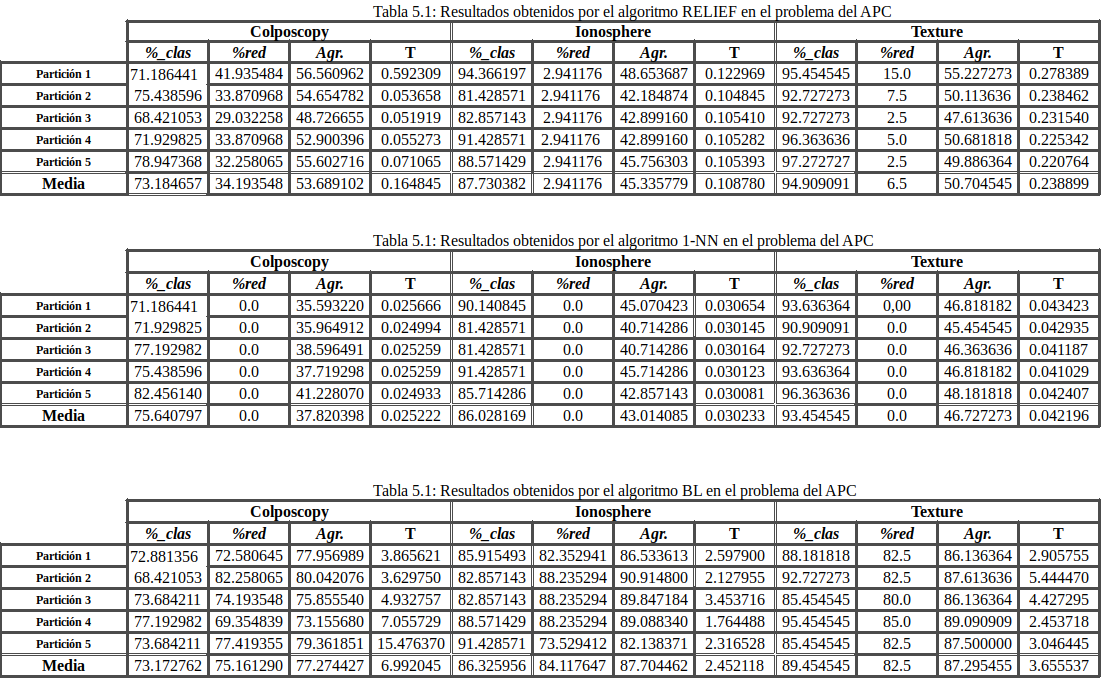
\includegraphics[width=1\linewidth]{screenshot004}
		\caption{}
		\label{fig:screenshot004}
	\end{figure}
	
	
	\subsubsection{Análisis de resultados practica 1}
	Como se ve en las tablas el la BL siempre gana en la función objetivo, esto es debido que obtiene una tasa de reducción muy superior a los otros dos algoritmos. Al tener el valor para calcular la función objetivo con 0.5 se le esta dando la misma importancia a reducir la tasa de acierto y la tasa de reducción. Por este motivo en términos de función objetivo el mejor algoritmos de estos tres es la BL. El problema de la BL es que en tasa de acierto no suele ser el mejor en ninguna de los conjunto de datos. Si no tenemos en cuenta la tasa de reducción no podríamos elegir un mejor algoritmo puesto que en unos conjuntos de datos salen vencedor el RELIEF y en otros el 1-NN, pero la diferencia entre el porcentaje de acierto entre uno u otro suele ser muy pequeño. La búsqueda local en este caso se suele situar muy cercano a los dos superando a algunas veces a uno de los dos. Pero nunca consigue situarse como el que mas tasa de acierto tiene.
	
	\subsubsection{Tiempos de ejecución resultados practica1 }
		El tiempo de ejecución de menor a mayor como era obvio el que menos tarda es el 1-nn puesto que los otros dos utilizan a este para la clasificación. Es prácticamente instantáneo
	
	Lo sigue el RELIEF que si el anterior tarda como el doble o triple que esta pero tampoco es un tiempo considerable.
	
	La búsqueda local es la mas lenta. Conseguí reducirla mucho al tener en cuenta que hay ocasiones en las que no hacia falta volver a valorar un peso porque no es posible que este mejore. Siendo los datos en lo que mas tarda los que mas número de características por elemento tienen.
	
	
	\subsubsection{Conclusión final resultados practica 1}
	No podríamos elegir uno entre los tres puesto que cada uno tiene sus puntos fuertes. Lo bueno de la búsqueda local es que reduciendo mas del doble que el RELIEF no perdemos mas de 5\% en el peor caso. Esto nos puede venir bien para saber que características de nuestros conjuntos son las que mas peso tienen a la hora de clasificar. En cambio siempre es superada por uno de los otros dos algoritmos como mínimo a la hora de clasificar los datos.

	\subsection{Análisis de AGG}
	\subsubsection{Tablas de AGG}
	Se tendrá una tabla con cada uno de los cruces realizado.
	\begin{figure}[H]
		\centering
		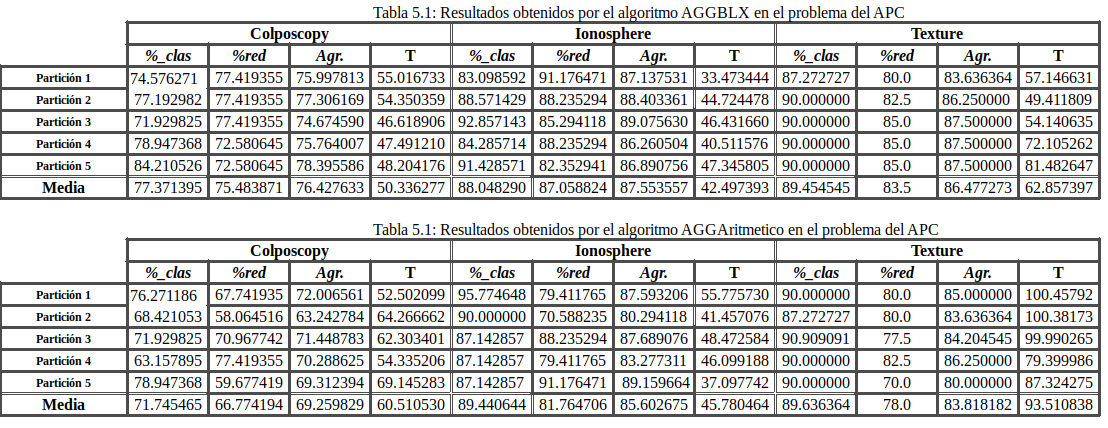
\includegraphics[width=1\linewidth]{screenshot005}
		\caption{}
		\label{fig:screenshot005}
	\end{figure}
	
	\subsubsection{Análisis de resultado AGG}
	En este caso el cruce BLX  es superior en función objetivo al cruce martinico al obtener entre un 3\% y 7\%. Quitando el conjunto de datos de colposcopy, en los demás los dos algoritmos están muy próximos en tasa de acierto. El problema del cruce aritmético es que reduce un poco peor que el BLX y al estar igualados en clase el BLX destaca un poco en la función objetivo al obtener mas reducción. BLX reduce mejor al permitir que los genes de los hijos puedan tener valores inferiores al mínimo de los padres. En cambio en el cruce aritmético esto no se puede dar. Para conseguir valores en los hijos menores que 0.2 uno de los genes de los padres tendría que ser menor a 0.2.
	
	En tasa de clase estan muy igualados en todos los conjuntos de datos menos en colposcopy donde el blx le saca un 6\%
	\subsubsection{Tiempos de ejecución de AGG}
	El tiempo de ejecución del cruce aritmético es superior a tiempo con el cruce blx. Esto es debido a que el cruce aritmético genera un mayor número de aleatorios (uno por cada gen del vector de pesos).
	\subsubsection{Conclusión final de AGG}
	En AGG me quedo con el cruce blx puesto que es mas rápido y siempre esta por encima en tasa de reducción y función objetivo. Ademas en los únicos casos en los que el aritmético ha gando al blx en tasa de clasificación ha sido por una diferencia menor a un 1\%
	
	\subsection{Análisis de AGE}
	Igual que en el apartado anterior compararemos los dos cruces pero esta vez para los algoritmos genéticos estacionarios.
	
	\subsubsection{Tablas de AGE}
	\begin{figure}[H]
		\centering
		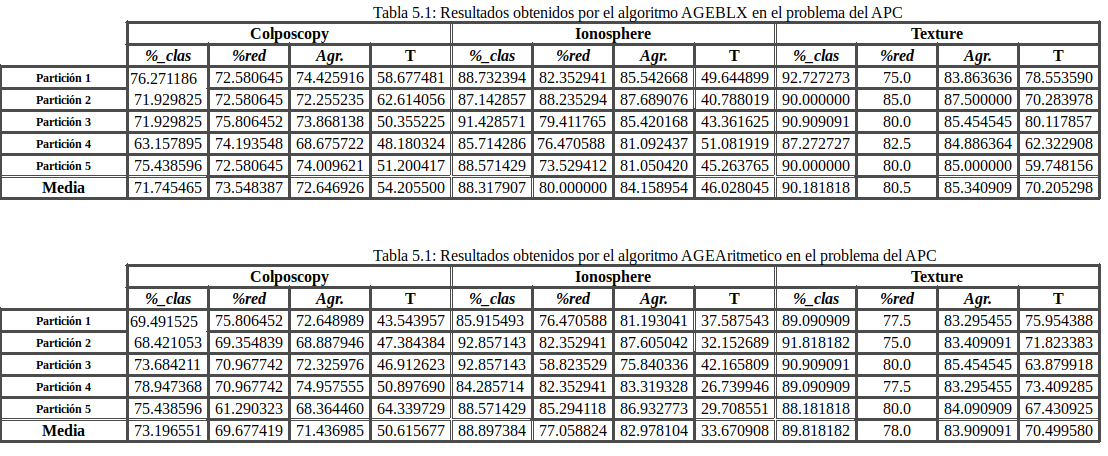
\includegraphics[width=1\linewidth]{screenshot006}
		\caption{}
		\label{fig:screenshot006}
	\end{figure}
	
	
	\subsubsection{Análisis de resultado AGE}
	En el generacional seguimos teniendo al cruce blx por encima del aritmético. Aunque en este caso están mucho mas próximo con una diferencia máxima en la función objetivo de un 2\%. En este caso la tasa de clase esta muy igualada, lo que marca esa pequeña diferencia es que el blx sigue teniendo una mejor tasa de reducción.
	
	\subsubsection{Tiempos de ejecución de AGE}
	En este caso los tiempos de ejecución son menores en el cruce aritmético que en el blx. Esto me hace pensear dos posibilidades. Esto podría darse por dos razones.
	\begin{enumerate}
		\item En las mediciones del AGGAritmético el procesador estaba sobrecargado por algunos procesos externos a la ejecución del scirpt.
		\item Generar un gran número de aleatorios de forma continuada al tener muchos mas cruces en el AGG que en el AGE se sobrecarga el procesador y por eso en el AGE reduce el tiempo. Si fuera esta opción podría tardar mas el cruce blx en el AGE debido a que tiene una mayor carga de operaciones y comprobaciones que el aritmético. 
	\end{enumerate}
	
	\subsubsection{Conclusión final de AGE}
	En este caso los dos algoritmos están muy igualados y cualquiera de los dos nos podría dar resultados muy parecidos aunque el cruce blx sigue siendo un poquito mejor.
	
	\subsection{Análisis de AGE vs AGG}
	Vamos a comparar los resultados sin tener en cuenta el tipo de cruce elegido. Lo que compararemos es si hay mejora entre el AGG y el AGE con el mismo cruce.
	\subsubsection{Tablas de AGE vs AGG}
	Vamos a comparar las medias obtenidas para los cuatro algoritmos.
	\begin{figure}[H]
		\centering
		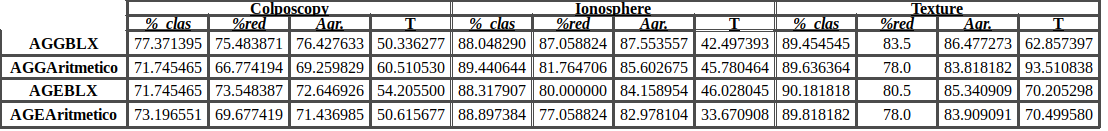
\includegraphics[width=1\linewidth]{screenshot008}
		\caption{}
		\label{fig:screenshot008}
	\end{figure}

	\subsubsection{Análisis de resultado AGE vs AGG}
	En este caso los algoritmos AGG son superiores en casi todos los caso que los algoritmos AGE. Esto puede darse a que en el AGG tengamos una mayor exploración al no estar obligando al algoritmos a sustituir siempre los hijos  nuevos si son mejores que los peores individuos de la poblacion. Esto hace que puedan entrar soluciones que en principio sean peores pero que puedan sacarnos de algún optimo local. 

	\subsubsection{Conclusión final AGE vs AGG}
	En este caso me quedaría con los algoritmos AGG y mas específicamente con el AGG	con cruce blx que esta un poquito por encima de las otras tres opciones.
	
	
	\subsection{Análisis de AM}
	\subsubsection{Tablas de AM}
	\begin{figure}[H]
		\centering
		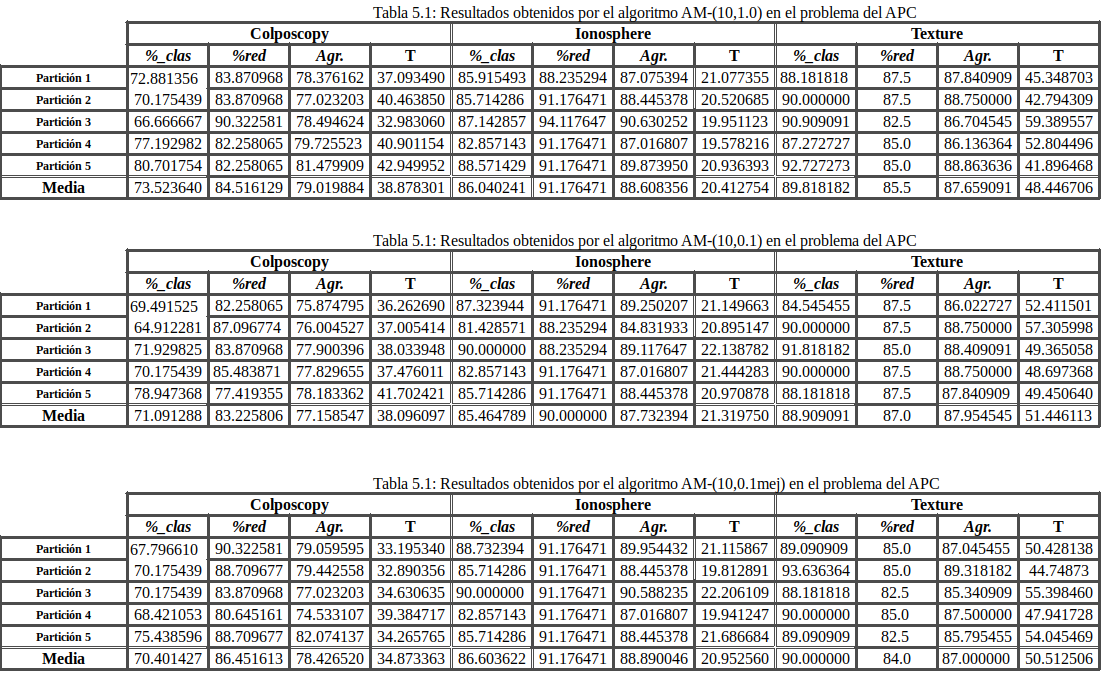
\includegraphics[width=1\linewidth]{screenshot009}
		\caption{}
		\label{fig:screenshot009}
	\end{figure}
	\subsubsection{Análisis de resultados AM}
	En este caso están todos muy igualados. Con una diferencia máxima de in 1\% en la función objetivo. Ninguno destaca por encima del otro en clasificación o en reducción. 
	
	\subsubsection{Tiempos de ejecución AM}
	En este apartados estamos igual que el apartado anterior. Ninguno destaca por encima de otro para poder decidir que uno de ellos es mas rápidos. Las diferencias que se dan son mínimas y podrían darse por una sobrecarga en le procesador.
	
	\subsubsection{Conclusión final AM}
	No propria elegir uno por encima de los demás puesto que tanto en tiempo como en función objetivo son prácticamente idénticos.
	
	\subsection{Análisis AM vs AG}
	\subsubsection{Tablas de AM vs AG}
	\begin{figure}[H]
		\centering
		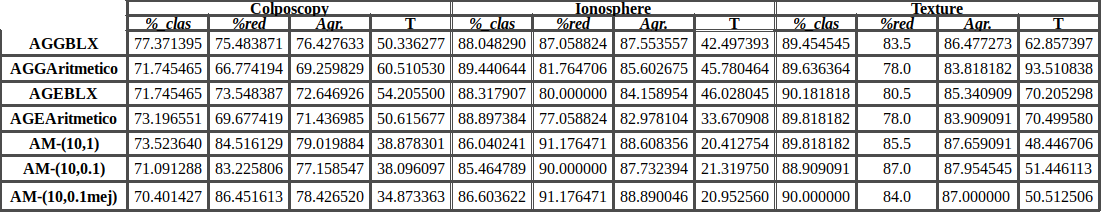
\includegraphics[width=1\linewidth]{screenshot010}
		\caption{}
		\label{fig:screenshot010}
	\end{figure}

	\subsubsection{Análisis de resultados AM vs AG}
	En este caso es muy claro que los vencedores en cuanto a función objetivo son los meméticos. Los tres algoritmos meméticos están siempre por encima de todos los algoritmos genéticos en función objetivo debido a que tienen de media un 3\% mas de tasa de reducción como mínimo al compararlo con el AGG con cruce blx que es el que mas se les aproxima. Esto se puede deber a que la búsqueda local con la mutación que tiene para generar vecinos conseguía una muy buena reducción. En cambio los AG están igualados o mejoran un poco la tasa de clasificación  de los AM. 
	
	\subsubsection{Tiempos ejecución AM vs AG}
	En este apartado si son claramente mejores los algoritmos memeticos puesto que las evaluaciones que utilizamos par ala búsqueda local son mucho menos costosas que realizar los torneos binarios, cruces y las mutaciones. Al perder evaluaciones en la búsqueda local realizaremos muchos menos ejecuciones del bucle y ahorramos unos 15 y 20 segundo. 
	
	\subsubsection{Conclusión final AM vs AG}
	Los algoritmos meméticos pierden un porcentaje muy pequeño de tasa de clasificación pero ganan en la tasa de reducción y tiempo con una diferencia mucho mayor.
	
	\subsection{Análisis de práctica 3}
	\begin{figure}[H]
		\centering
		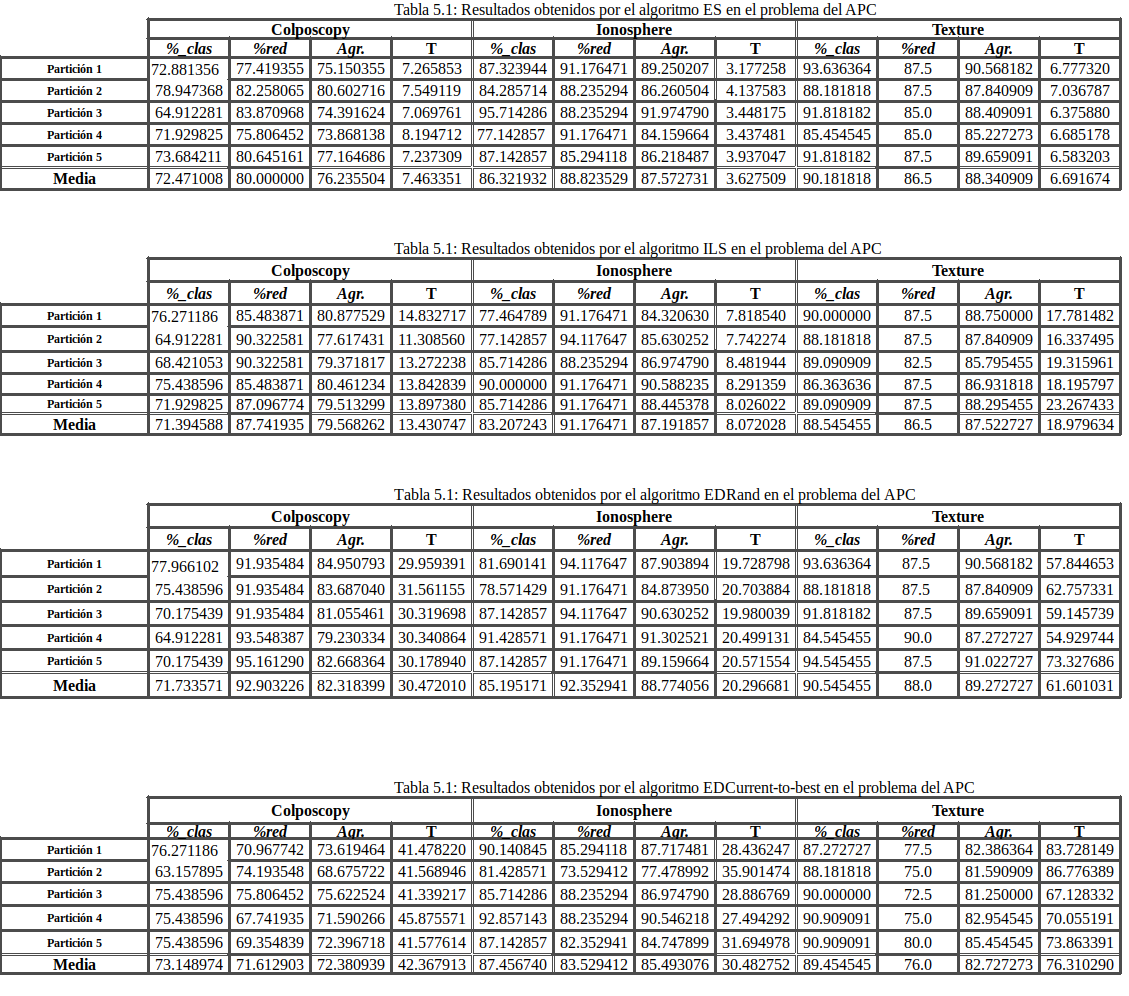
\includegraphics[width=1\linewidth]{screenshot013}
		\caption{}
		\label{fig:screenshot013}
	\end{figure}
	
	
	\subsubsection{Análisis de resultados}
	
	
	
	
	
	
	
	\section{Bibliografía}
	No he usado nada fuera de las propias paginas de información de python o de las librerías utilizadas como podría ser la de numpy.
	
	\
  
\end{document}